\chapter{Prototypical Implementation}
\label{ch:prototype}

\vspace{-1cm}
\begin{center}
Eduard Hirsch
\end{center}

\section{Architecture}

The core architecture of the INTERLACE project presented next is multi-layered and concentrates on being scalable and highly distributable in contrast to the current monolithic payment platform used by Sardex.

The chosen block-chain approach is going to be explained in detail. The technical challenges during the planning of that implementation strategies are discussed in subsequent sections of that chapter.

\subsection{Sardex Network}

In deliverable D2.1 and D3.1 the current architecture has been written down using the AS(I)M approach and as mentioned before a working client-server application based on message-passing has been developed. This application was realized using the ICEF-framework which is founded on abstract state machines applying a programming language similar to ASM logic definitions.

That classic model was used to derive a new payment network based on block-chain approach. The thoughts for the new network comprise using a publicly maintained and an easy to use block-chain which supports the idea of a interest-free mutual credit system enabling account based balances rather than token based currencies only. These thoughts led to a prototypical implementation using hyperledger fabric together with hyperledger composer.

Regardless of the choice of hyperledger environment it also has been important having central payment network which is not only reliable and verifiable but also to a specific extend controllable in order to impose the basic Sardex payment rules on it..

\subsection{Hyperledger Fabric Network}

The given network constraints were used while creating a new hyperledger fabric network which sets up a core environment offering a basic block-chain to interact with. Next a close look is taken on the actual implemented network and a description for the various parts is given.

In figure \ref{fig:prototype-net} the current working environment is shown. It is utilising the possibilities hyperledger fabric is offering. When looking further into detail fabric actually imposes a structure to a newly created network for which the following main components can be singled out when focusing on Interlace:

\begin{itemize}
	\item Sardex as participating Organisation
		\subitem One peer (named: peer0.sardex.sardex.net)
		\subitem Clients and Services connecting to the network
		\subitem Sardex Member Ship Provider (SardexMSP)
	\item An orderer managed by "Interlace" Organisation
		\subitem An orderer (named: orderer.sardex.net)
		\subitem Interlace Member Ship Provider (InterlaceOrdererMSP)
	\item Certification Authority (CA)
\end{itemize}

Starting from a Certification Authority (CA) a user may issue a unique identity which can be verified any time by anyone participating in the network. Those identities are part of the process of giving members of the circuit right to work with and facilitate the network with particular roles and access privileges. The actual empowering of a user takes place inside of the membership provider.

Nevertheless, the power of an MSP goes beyond simply caring about who is a network participant or member of a particular channel. An MSP is able of identifying specific roles an actor might play either within the scope of the organization the MSP represents (e.g., admins, or as members of a sub-organization group), and defines the foundation for giving access privileges in the context of a network and channel (e.g., channel admins, readers, writers). More details can be found on the documentations web-site of hyperledger fabric\footnote{https://hyperledger-fabric.readthedocs.io/en/master/membership/membership.html}.

Due to simplicity reasons and in order to set-up the prototype network quickly, access/role management has been reduced to a minimum. Section \ref{sec:id-management} focus on a more detailed explanation on how those things might work in or might be changed to in case of large scale scenarios.  


\begin{figure}[htbp]
  \centering
  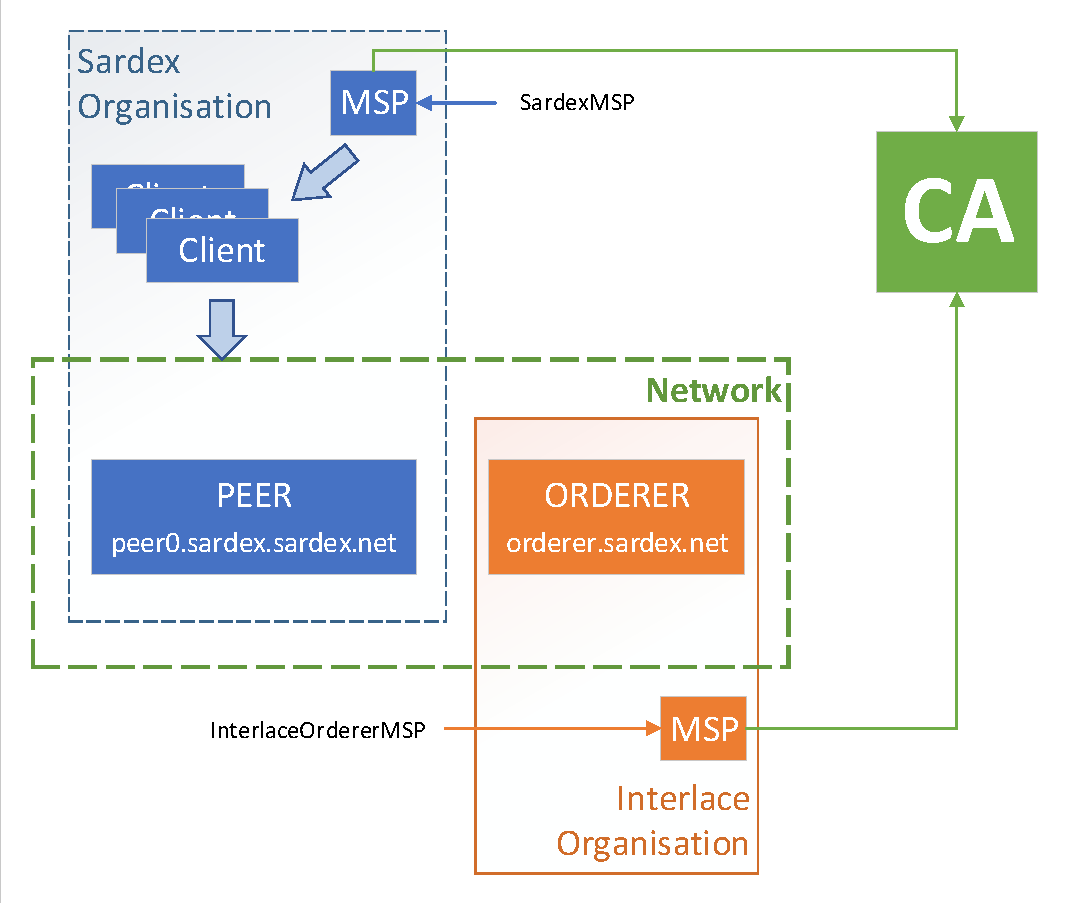
\includegraphics[width=0.5\textwidth, clip, trim=1mm 1mm 1mm 1mm]{Figures/basic-network}
  \caption{\bf\small Network Structure implemented by the Prototype}
  \label{fig:prototype-net}
\end{figure}

\begin{figure}[htbp]
  \centering
  %\includegraphics[width=1.0\textwidth]{Figures/TODO}
  \caption{\bf\small TODO: Extended Network Structure}
  \label{fig:prototype-net-ext}
\end{figure}

\subsection{cto-model}

\section{Prototype}

The prototype is a block-chain realisation of INTERLACE, can be found on GitHub\footnote{https://github.com/InterlaceProject/InterlaceBlockchain} and is based on the specifications created in deliverable D3.1\cite{INTERLACE_D31} as well as the ASIM Specification of the requirements.

First it is necessary to install the pre-requisites which are available for Linux and Mac OS. Currently these are the recommended operating systems, however, with additional effort it might be possible to run the INTERLACE blockchain on Windows directly. To support windows user a virtual machine set-up is also available.

Additionally, it is also important to set-up a development environment described at the composer GitHub repository. If you do not want to set up the complete environment it would be still recommended to install and start Composer Playground. Playground enables you to connect, alter and test the INTERLACE payment network. Nevertheless, playground is not required and you might use composer-cli or other methods to utilized the network.

\subsection{Install}

This part of the documents talks about how to set-up and run the business network on your machine. However, before it is actually possible to begin it is necessary to install the pre-requisites which are listed at the hyperledger composer documentation\footnote{https://hyperledger.github.io/composer/latest/installing/installing-prereqs.html}. The website also offers a download where a script for installing all the requirements for a machine is provided.

Nevertheless, for windows user those script won't help because for now most of the packages are not yet prepared (as of writing) for a windows operating systems. For this user group a virtual machine has been prepared which is also installing all the necessary frameworks and software tools during provisioning. This virtual machine is controlled by vagrant\footnote{https://www.vagrantup.com/} and uses hyper-v or virtual box as hypervisor (two different branches). That VM configuration is published at GitHub\footnote{https://github.com/hirsche/hyperledger}.

\textbf{Environment Start-Up}

Once the hyperledger environment is installed, the next step is about starting the INTERLACE environment. To make communication uniform the block-chain is configured to publish all services under the host name "interlace.chain". Windows user facilitating the suggested vagrant set-up the new hostname is added to your host-file during start-up time using the vagrant-hostmanager plug-in. Thus there is no need to configure the name manually.

\textbf{Configure Hostnames}

For non-vagrant users it is important before executing for the local set-up to add a host name entry for "interlace.chain". Usually this entry will point to ip 127.0.0.1 (localhost). On a production system or if it was chosen to start the hyperledger composer services on a public interface, the IP needs to be fixed accordingly. Here is a list of hosts-file locations according to different operating systems types:

\begin{itemize}
	\item Mac OS: /private/etc/hosts
    \item Linux: /etc/hosts
    \item Windows: C:\textbackslash Windows\textbackslash System32\textbackslash drivers\textbackslash etc\textbackslash hosts
\end{itemize}

The format may vary a little but usually a new host with its hostname is defined using it's IP and the desired host name like

\begin{lstlisting}
	127.0.0.1        interlace.chain
\end{lstlisting}

Depending on the operating system it might be also necessary to update and restart the respective services (e.g. MacOS).

\textbf{Run fabric block chain (the first time)}

Now the main configurations have been done and hyperledger fabric can be started, which acts as a base for hyperledger composer. To continue the GitHub repository \footnote{https://github.com/InterlaceProject/InterlaceBlockchain} if not yet done needs to be downloaded by using the git visioning system by calling

\begin{lstlisting}[language=bash]
	git clone https://github.com/InterlaceProject/InterlaceBlockchain.git
\end{lstlisting}

In the created directory "InterlaceBlockchain" the business network implementation including a web application can be found. The next listing shows the bash script which downloads several fabric docker container and finally starts them using docker-composer \footnote{https://docs.docker.com/compose/}:

\begin{lstlisting}[language=bash]
	cd fabric
	./downloadFabric.sh # updates images - only the first time necessary
	./startFabric.sh # start up docker environment using docker-compose
\end{lstlisting}

\textbf{Initialize Interlace-Chain}

Finally, after fabric has been started the next step is to initialize the block chain with a call of

\begin{lstlisting}[language=bash]
	cd chain
	./initNetwork.sh # use hyperledger composer to create a business network and deploy it
\end{lstlisting}

\textbf{./initNetwork.sh} will copy all models and script to the network peers to make them accessible in the hyperledger blockchain. The last step in the script starts the business network.

You may further use playground to access and test Credit- or DebitTransfer transactions. \textbf{data.json} should act as a helper to init the network by hand, but it is recommended to update the JavaScript function \textit{initBlockchain(transfer)} in \textit{./chain/lib/init.js}. That chain-code part is executed when transaction InitBlockchain is submitted. Be careful to run \textbf{InitBlockchain} only once otherwise errors or duplicate entries might happen resulting in a inconsistent chain.

\textbf{Network updates after chain-code changes}

After changes to the acl, cto, queries, the libraries or other parts of the core chain-code application the network needs to be updated. This can be achieved by executing

\begin{lstlisting}[language=bash]
	cd chain
	./updateNetwork.sh
\end{lstlisting}

This script reads the current version number of \textit{package.json} file increases it by one and creates a new bna package. When scripts are correct and the bna-package could be created it is deployed to the peers and the network updated to a new, higher network version which will utilize the new bna package.

\textbf{Shutting down}

Sometimes it is useful to throw away everything and restart from scratch. To tear down fabric and remove card left-overs execute:

\begin{lstlisting}[language=bash]
	cd fabric
	./teardownFabric.sh
	./deletePlaygroundCards.sh
\end{lstlisting}

\textbf{Start a rest server}

Once the network is running (no playground needed) it is also possible to start a HTTP-Server which allows to interact with the network over REST. The script

\begin{lstlisting}[language=bash]
	cd chain
	./startRestServer.sh
\end{lstlisting}

starts the server and allows to get an overview of the restful interface by opening

\begin{lstlisting}
http://interlace.chain:3000/explorer
\end{lstlisting}

in a browser. The REST interface itself may be contacted over

\begin{lstlisting}
http://interlace.chain:3000/
\end{lstlisting}

when using it together with an external application. In case you didn't set-up the host interlace.chain in your hosts file and you are running all the services locally without a VM you might also use localhost instead of interlace.chain as host name.

\subsection{Working with the environment}

Next a closer look is taken on how the environment might be facilitated using different approaches. It is possible to connect to the chain using composer-cli, taking advantage of composer playground (the graphical interface) or use the simple web-front-end created for the project.

\textbf{Start and test network with playground}

If you've decided to install and use Composer Playground it can be started using that command

\begin{lstlisting}[language=bash]
	composer-playground
\end{lstlisting}

The standard configuration opens a browser connecting to playground at localhost with port 8080. If you've running playground in a separate virtual environment like e.g. in a docker container, it may be necessary to start the browser manually, determine the VM-/Containers-IP and fill in the address manually in the URL field.

\todo{screenshots of playground}

\textbf{Run Transactions with composer-cli}

Init network transaction:

\begin{lstlisting}[language=bash]
	composer transaction submit -c admin@sardex-open-network -d  '{ "$class": "net.sardex.interlace.InitBlockchain" }'
\end{lstlisting}

The InitBlockchain transaction is setting up some basic accounts as well as demo members to continue with simple transactions right away.

Submit a credit transfer from account a1 to a2 with amount of 800 SRD:

\begin{lstlisting}[language=bash]
	composer transaction submit -c admin@sardex-open-network -d  '{ "$class": "net.sardex.interlace.CreditTransfer", "amount": 800, "senderAccount": "resource:net.sardex.interlace.CCAccount#a1", "recipientAccount": "resource:net.sardex.interlace.CCAccount#a2" }'
\end{lstlisting}

Submit a debit transfer from account a1 to a2 with amount of 200 SRD:

\begin{lstlisting}[language=bash]
	composer transaction submit -c admin@sardex-open-network -d  '{ "$class": "net.sardex.interlace.DebitTransfer", "amount": 200, "senderAccount": "resource:net.sardex.interlace.CCAccount#a1", "recipientAccount": "resource:net.sardex.interlace.CCAccount#a2" }'
\end{lstlisting}

A successful debit transfer creates a PendingTransfer entry with status Pending containing an OTP (one time pad). This OTP can be used by the debitor to confirm the transaction. Thus in the next example "995317396" is used to call a transaction DebitTransferAcknowledge to acknowledge the debit transfer:

\begin{lstlisting}[language=bash]
	composer transaction submit -c admin@sardex-open-network -d  '{ "$class": "net.sardex.interlace.DebitTransferAcknowledge", "transfer": "resource:net.sardex.interlace.PendingTransfer#995317396" }'
\end{lstlisting}

\textbf{The web front-end}

The web front-end currently is a simple web site generated by a yeoman generator provided by the composer-community. The web application can be found in the webapp directory.

In order to get the web application to run properly it is necessary to start-up the whole network and start the REST-server as described in the previous steps.

The web app which is based on AngularJS needs various node.js packages downloaded and installed which is achieved by calling

\begin{lstlisting}[language=bash]
	cd webapp
	npm install
\end{lstlisting}

After that a development server can be started by calling

\begin{lstlisting}[language=bash]
	cd webapp
	npm start
\end{lstlisting}

npm will start a web server at port 4200. If you work locally it also tries to open a browser which is showing the web application, otherwise you'd need start a browser manually and enter the URL by yourself. This is the URL where the server can be reached:

\begin{lstlisting}
http://interlace.chain:4200
\end{lstlisting}

The web page is based on AngularJS and communicates over REST with our previously started REST server facilitating asynchronous AJAX-request.

\section{Technical Details}

TODO

\section{Identity Management}
\label{sec:id-management}

TODO

---------------

\todo{outline:}
\begin{verbatim}

Sec: Architecture:
  - Sardex Network
  - fabric network  
  - cto-model 
    
Sec: Prototype
    - installation
    - usage
    
Sec: Technical Details:
    - chain-code bits
    - queries
    - acl-file
    - deployment
    - web application
    - docker-compose
    - rest server https://hyperledger.github.io/composer/latest/reference/rest-server

Sec: Identity Management Considerations:
  - permissions
  - https://www.codementor.io/gangachris125/passport-jwt-authentication-for-hyperledger-composer-rest-server-jqfgkoljn
  - passport.js (swagger) www.passportjs.org/docs/
  - user profile strategies

\end{verbatim}
